\documentclass{standalone}
\usepackage{tikz}
\usetikzlibrary{positioning, shapes.geometric}
\usepackage{amsfonts}
\begin{document}

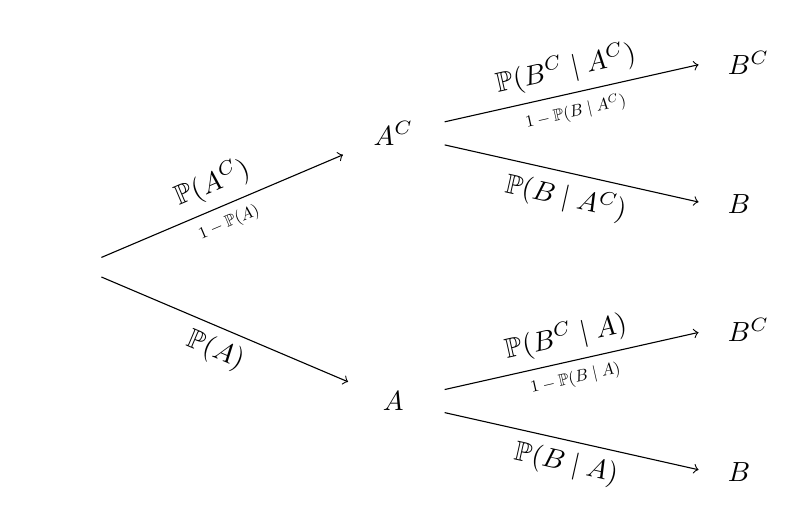
\begin{tikzpicture}[->, grow=right, sloped,
level 1/.style={sibling distance=3.4cm, level distance=4cm},
level 2/.style={sibling distance=1.8cm, level distance=4cm},
level 3/.style={sibling distance=0.6cm,},
level 4/.style={sibling distance=0.4cm,}]
\tikzstyle{bag} = [text width=3em, text centered] % Define bag style
\tikzstyle{end} = [text width=0em, text centered] % Define end style

\node[bag] {} % Root node with bag style
    child {
        node[bag] {$A$} % Bag node
            child {
                node[end, label=right: {$B$}] {} % End node with label
                edge from parent
                node[above] {} % Label above the edge
                node[below] {$\mathbb{P}(B \mid A)$} % Label below the edge
            }
            child {
                node[end, label=right: {$B^C$}] {} % End node with label
                edge from parent
                node[above] {$\mathbb{P}(B^C \mid A)$} % Label above the edge
                node[below] {\scalebox{0.6}{$1-\mathbb{P}(B \mid A)$}} % Label below the edge
            }
            edge from parent 
            node[above] {}
            node[below] {$\mathbb{P}(A)$} % Label below the edge
    }
    child {
        node[bag] {$A^C$} % Bag node
            child {
                node[end, label=right: {$B$}] {} % End node with label
                edge from parent
                node[above] {} % Label above the edge
                node[below] {$\mathbb{P}(B \mid A^C)$} % Label below the edge
            }
            child {
                node[end, label=right: {$B^C$}] {} % End node with label
                edge from parent
                node[above] {$\mathbb{P}(B^C \mid A^C)$} % Label above the edge
                node[below] {\scalebox{0.6}{$1-\mathbb{P}(B \mid A^C)$}} % Label below the edge
            }
            edge from parent         
            node[above] {$\mathbb{P}(A^C)$} % Label above the edge
            node[below] {\scalebox{0.6}{$1-\mathbb{P}(A)$}} % Label below the edge
    };
\end{tikzpicture}

\end{document}
